

\chapter{Benchmarking of Asynchronous Data Processing Algorithms}
\label{cha:a_short_latex_tutorial_with_examples}

In this chapter, we delve into the benchmark results of two key algorithms applied using various strategies and implementations. These algorithms can be understood as abstract representations of real-world tasks that involve processing large amounts of data asynchronously. The two main algorithms under consideration are:

\begin{enumerate}
\item Finding the largest word in a set of files
\item Grouping of words based on their sizes, known as the "group words" operation
\end{enumerate}

The "group word" operation identifies words within a specified size range in a dataset. The algorithm then returns a collection of these words, along with a count of their occurrences, and is particularly designed to output the most recurring words within the specified range. This operation presents an intriguing computational challenge as it requires efficient data retrieval, processing, and frequency analysis.

Conversely, finding the largest word in a set of files, although seemingly simple, becomes a non-trivial task when considering vast amounts of data.

The data used in these tests is a collection of text files from Project Gutenberg, a large digital library of thousands of free eBooks. Project Gutenberg offers a wide variety of books in different languages, and for this experiment, we used a random sample of hundreds of books, providing a diverse and challenging dataset for our implementations.

During the implementations, a conscious effort was made to keep the operation pipelines as similar as possible across the different technologies for each algorithm. This endeavor aimed to create a fair and representative evaluation of the behaviors of each technology. By maintaining consistency in pipeline operations, we can more accurately attribute performance differences to the underlying technology, rather than variations in the implemented code. This approach brings us closer to a true comparison of how each technology handles the challenges of asynchronous I/O data retrieval and processing.

In certain instances, particularly with Java, there was a need to incorporate external libraries for non-blocking asynchronous file retrieval. This requirement highlights the varying degrees of native support for these operations across programming environments. Some environments have native functions, while others rely heavily on third-party solutions. This aspect of the project mirrors the challenges often faced in real-world environments, where the necessity to adapt and find suitable solutions is a common part of the development process.

The implementations differ in the specific programming languages, libraries, and technologies they use. This allows us to evaluate the relative strengths and weaknesses of each approach and provides valuable insights into how these factors can affect performance.

After presenting and discussing each implementation and its results, we will be able to directly compare them. This will enable us to draw meaningful conclusions about the performance of the strategies and technologies when applied to the same task under the same conditions. Specifically, we are interested in how the performance of a given strategy or technology can vary across different programming frameworks when tasked with finding the largest word and executing the group word operation.

\section{.NET Implementation}
\label{sec:dotnet_implementation}
\begin{table}[h!]
    \centering
    \resizebox{\textwidth}{!}{%
    \begin{tabular}{|l|c|c|}
    \hline
    \textbf{Strategy} & \textbf{Processing Time Average Run 1 (ms)} & \textbf{Processing Time Average Run 2 (ms)} \\ \hline
    RunCountWordsBaseline & 63765.67 & 49880.33 \\ \hline
    RunSyncTest & 43921.67 & 36062.67 \\ \hline
    RunAsyncEnumerableTest & 62422 & 57870 \\ \hline
    RunRxTest & 46833.33 & 37015.66 \\ \hline
    \end{tabular}%
    }
    \caption{Processing times for different strategies for "Count Words".}
    \label{tab:strategies_times_count_words}
\end{table}

\begin{figure}[H]
    \raggedright
    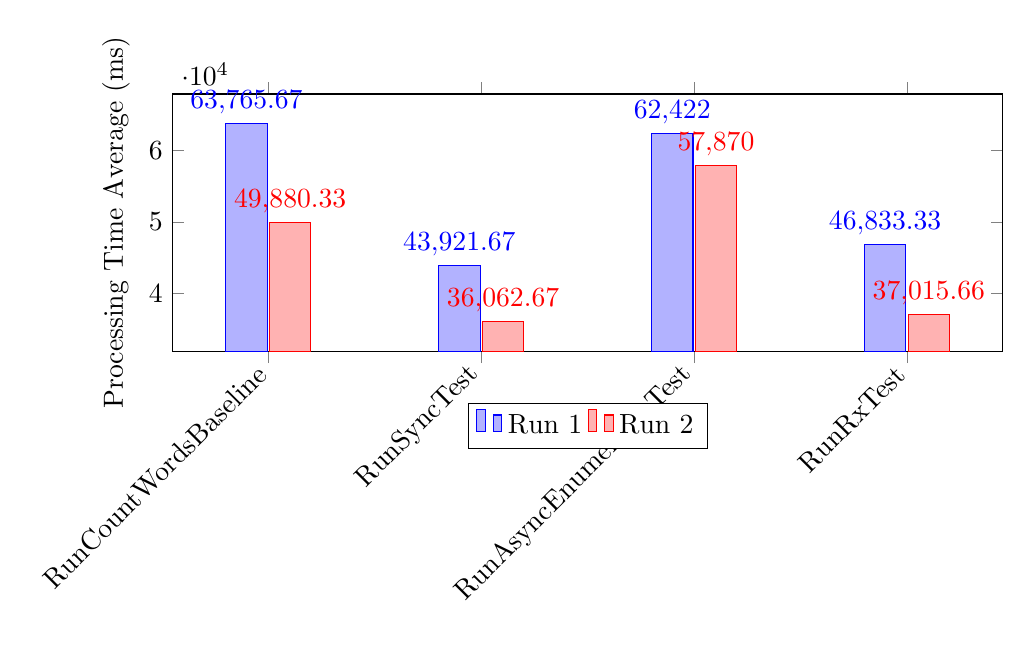
\begin{tikzpicture}
    \begin{axis}[
        ybar=2*\pgflinewidth,
        width=1.0\textwidth,
        height=0.4\textwidth,
        bar width=15pt,
        enlargelimits=0.15,
        legend style={at={(0.5,-0.2)}, anchor=north, legend columns=-1},
        ylabel={Processing Time Average (ms)},
        symbolic x coords={RunCountWordsBaseline, RunSyncTest, RunAsyncEnumerableTest, RunRxTest},
        xtick=data,
        xticklabel style={rotate=45,anchor=east},
        nodes near coords,
        nodes near coords align={vertical},
        ]
    \addplot coordinates {(RunCountWordsBaseline, 63765.67) (RunSyncTest, 43921.67) (RunAsyncEnumerableTest, 62422) (RunRxTest, 46833.33)};
    \addplot coordinates {(RunCountWordsBaseline, 49880.33) (RunSyncTest, 36062.67) (RunAsyncEnumerableTest, 57870) (RunRxTest, 37015.66)};
    \legend{Run 1, Run 2}
    \end{axis}
    \end{tikzpicture}
    \caption{Processing times for different strategies for "Count Words" for two runs.}
    \label{fig:count_words_processing_times}
\end{figure}


\section{Java/Kotlin Implementation}
\label{sec:java_implementation}

In this section, we will present the different strategies utilized in Java and Kotlin implementations for file processing and compare their performances. In the case of Java, asynchronous file reading isn't directly supported by the standard libraries. To overcome this limitation and maintain parity with the other implementations, we made use of a library named \texttt{AsyncFiles}. This library was developed by Professor Jorge Martins of the Lisbon Engineering Superior Institute. It provides an efficient and straightforward way to perform asynchronous file reading operations in Java.

\subsection{Strategies}
\label{subsec:strategies}


\subsubsection{Kotlin Flow}
\label{subsubsec:kotlin_flow}
The Kotlin Flow strategy is based on the concept of 'flows' in the Kotlin Coroutines library. A Flow is an asynchronous data stream that sequentially emits values and completes normally or with an exception. The concept of a flow is very similar to that of Reactive Streams, which emphasizes data streams and the propagation of change.

\subsubsection{Java Reactor (Flux)}
\label{subsubsec:java_reactor_flux}
Reactor is a fourth-generation reactive library, based on the Reactive Streams specification, for building non-blocking applications on the JVM based on Java 8 and later. This strategy uses the Flux class, a Reactive Streams Publisher with rx operators that emits 0 to N elements, and then completes (successfully or with an error).

\subsubsection{RxJava (Observable)}
\label{subsubsec:rxjava_observable}
RxJava is a Java VM implementation of Reactive Extensions: a library for composing asynchronous and event-based programs by using observable sequences. The Observable class, when subscribed, emits items or signals of any kind to the observer. 

\subsubsection{Blocking Reader in Streams}
\label{subsubsec:blocking_reader_streams}
This strategy uses the Java's streams interface to read the data in a blocking manner. Due to the blocking nature of the I/O operations, this approach may lead to slower processing times as it has to wait for each I/O operation to complete.

\subsubsection{MultiThread}
\label{subsubsec:multithread}
The MultiThread strategy leverages the Java's built-in thread support to process data concurrently. By distributing the work across multiple threads, it often results in improved performance, especially for CPU-bound tasks.

\subsubsection{Concurrency with Kotlin Flow}
\label{subsubsec:concurrency_kotlin_flow}
This strategy is an enhancement of the Kotlin Flow approach where data processing is performed concurrently. By using the built-in concurrency support in the Kotlin Coroutines library, it aims to improve the performance of data processing.

\subsubsection{RxJava with Concurrency (Observable)}
\label{subsubsec:rxjava_concurrency_observable}
This strategy is a concurrent version of the RxJava Observable approach. It uses the concurrency features in the RxJava library, such as Schedulers, to improve the performance of data processing.

\subsubsection{Blocking Reader in Streams with Concurrency}
\label{subsubsec:blocking_reader_streams_concurrency}
This strategy is a concurrent adaptation of the Blocking Reader in Streams strategy. It attempts to mitigate the blocking delays by processing multiple streams concurrently using multiple threads.

\subsubsection{Baseline}
\label{subsubsec:baseline}
The Baseline strategy is a straightforward implementation without any pipelining or other overhead. It serves as a reference for comparison. This method may use traditional synchronous I/O operations and sequential processing.

\subsubsection{Sequential Processing with Kotlin Flow}
\label{subsubsec:sequential_processing_kotlin_flow}
This is a variant of the Kotlin Flow strategy, but with sequential processing. The idea is to demonstrate the performance difference when the same operations are performed in sequence, rather than concurrently.

\subsubsection{IO Blocking Operations}
\label{subsubsec:io_blocking_operations}
This strategy represents a traditional approach to dealing with I/O operations - blocking until each operation is complete. It often results in slower processing times due to the time spent waiting for I/O tasks.


\subsection{Results}
\label{subsubsec:results}

\subsubsection{Biggest Word Results}
\label{subsubsec:biggest_word_results}

\begin{table}[h!]
    \centering
    \resizebox{\textwidth}{!}{%
    \begin{tabular}{|l|c|}
    \hline
    \textbf{Strategy} & \textbf{Processing Time Average (ms)} \\ \hline
    NIO Reactor Flux & 1148 \\ \hline
    NIO Reactor Flux with Concurrency (use of \texttt{parallel()}) & 1002 \\ \hline
    NIO Observable RXJava & 945 \\ \hline
    NIO Observable with Concurrency (use of \texttt{parallel()})& 841 \\ \hline
    Blocking Reader in Streams & 3897 \\ \hline
    Blocking Reader MultiThread  & 691 \\ \hline
    Blocking Reader Streams with Concurrency & 3011 \\ \hline
    NIO Baseline & 912 \\ \hline
    Concurrent Processing with Kotlin Flow & 2435 \\ \hline
    Sequential Processing with Kotlin Flow & 5050 \\ \hline
    Kotlin Flow IO Blocking Operations & 5216 \\ \hline
    \end{tabular}%
    }
    \caption{Processing times for different Java/Kotlin strategies for "Biggest Word".}
    \label{tab:strategies_times_biggest_word}
    \end{table}
    
   
    \begin{figure}[H]
        \raggedright
        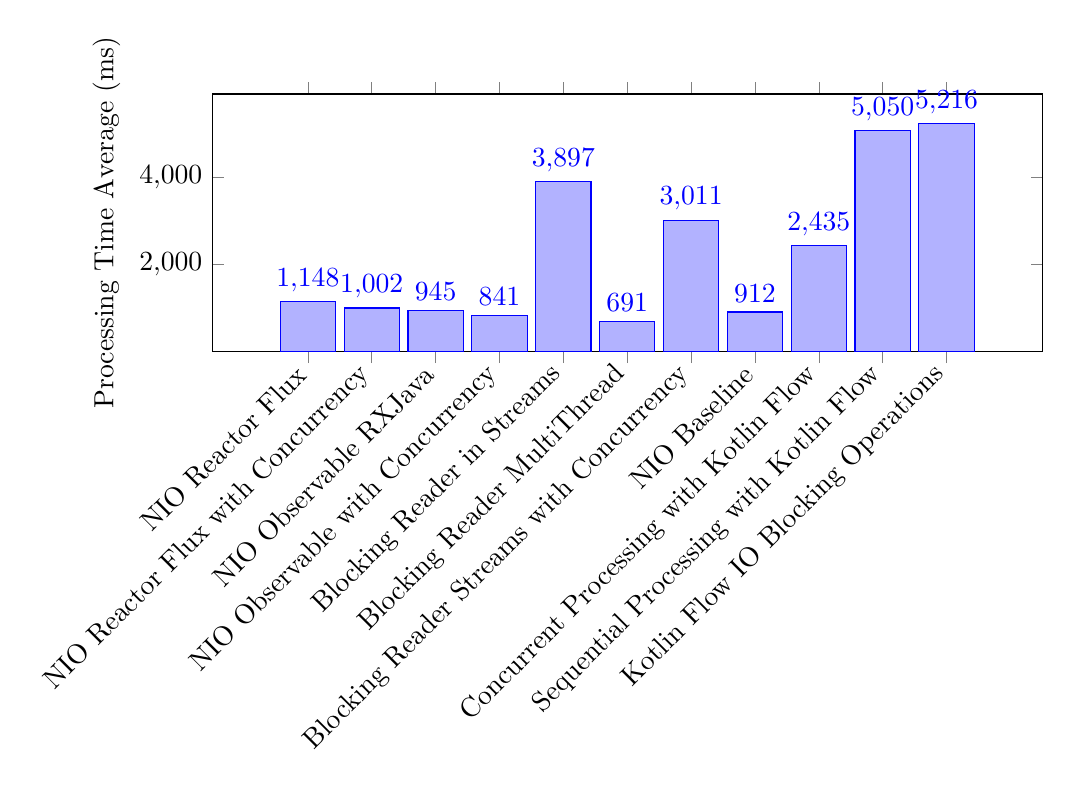
\begin{tikzpicture}
        \begin{axis}[
            ybar=2*\pgflinewidth,
            width=1.0\textwidth,
            height=0.4\textwidth,
            bar width=20pt,
            enlargelimits=0.15,
            legend style={at={(0.5,-0.2)}, anchor=north, legend columns=-1},
            ylabel={Processing Time Average (ms)},
            symbolic x coords={NIO Reactor Flux, NIO Reactor Flux with Concurrency, NIO Observable RXJava, NIO Observable with Concurrency, Blocking Reader in Streams, Blocking Reader MultiThread, Blocking Reader Streams with Concurrency, NIO Baseline, Concurrent Processing with Kotlin Flow, Sequential Processing with Kotlin Flow, Kotlin Flow IO Blocking Operations},
            xtick=data,
            xticklabel style={rotate=45,anchor=east},
            nodes near coords,
            nodes near coords align={vertical},
            ]
        \addplot coordinates {(NIO Reactor Flux, 1148) (NIO Reactor Flux with Concurrency, 1002) (NIO Observable RXJava, 945) (NIO Observable with Concurrency, 841) (Blocking Reader in Streams, 3897) (Blocking Reader MultiThread, 691) (Blocking Reader Streams with Concurrency, 3011) (NIO Baseline, 912) (Concurrent Processing with Kotlin Flow, 2435) (Sequential Processing with Kotlin Flow, 5050) (Kotlin Flow IO Blocking Operations, 5216)};
        \end{axis}
        \end{tikzpicture}
        \caption{Processing times for different Java/Kotlin strategies for "Biggest Word".}
        \label{fig:biggest_word_processing_times}
    \end{figure}
    

    
    \subsubsection{Group Word Results}
    \label{subsubsec:group_word_results}
    
    \begin{table}[h!]
    \centering
    \resizebox{\textwidth}{!}{%
    \begin{tabular}{|l|c|}
    \hline
    \textbf{Strategy} & \textbf{Processing Time Average (ms)} \\ \hline
    GroupWordsBaseline & 4420 \\ \hline
    GroupWordsRXJava & 7531 \\ \hline
    GroupWordsInRectorCoreFlux & 9074 \\ \hline
    GroupWordsBlockingReaderInMultiThread & 7850 \\ \hline
    GroupWordsBlockingReaderInStreams & 7323 \\ \hline
    GroupWordsWithFlow (Kotlin) & 15021 \\ \hline
    \end{tabular}%
    }
    \caption{Processing times for different Java/Kotlin strategies for "Group Words".}
    \label{tab:strategies_times_group_words}
    \end{table}
    
    \begin{figure}[H]
        \centering
        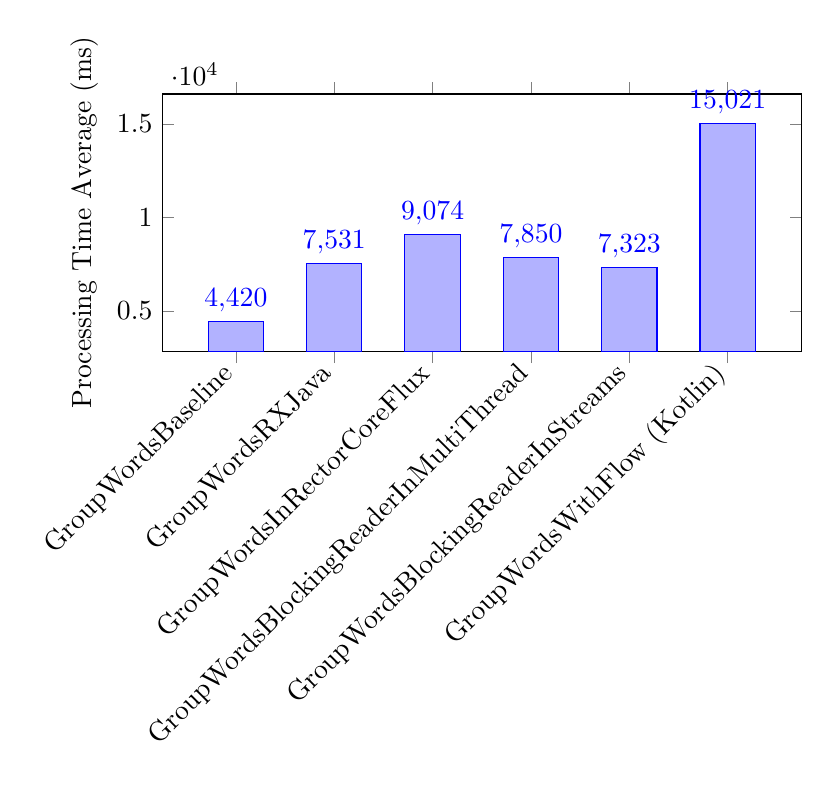
\begin{tikzpicture}
        \begin{axis}[
            ybar=2*\pgflinewidth,
            width=0.8\textwidth,
            height=0.4\textwidth,
            bar width=20pt,
            enlargelimits=0.15,
            legend style={at={(0.5,-0.2)}, anchor=north, legend columns=-1},
            ylabel={Processing Time Average (ms)},
            symbolic x coords={GroupWordsBaseline, GroupWordsRXJava, GroupWordsInRectorCoreFlux, GroupWordsBlockingReaderInMultiThread, GroupWordsBlockingReaderInStreams, GroupWordsWithFlow (Kotlin)},
            xtick=data,
            xticklabel style={rotate=45,anchor=east},
            nodes near coords,
            nodes near coords align={vertical},
            ]
        \addplot coordinates {(GroupWordsBaseline, 4420) (GroupWordsRXJava, 7531) (GroupWordsInRectorCoreFlux, 9074) (GroupWordsBlockingReaderInMultiThread, 7850) (GroupWordsBlockingReaderInStreams, 7323) (GroupWordsWithFlow (Kotlin), 15021)};
        \end{axis}
        \end{tikzpicture}
        \caption{Processing times for different Java/Kotlin strategies for "Group Words".}
        \label{fig:processing_times}
        \end{figure}

... 
% Here you conclude the entire chapter by summarizing your findings and interpretations.


\section{JavaScript Implementation}
\label{sec:js_implementation}
\begin{table}[h!]
    \centering
    \resizebox{\textwidth}{!}{%
    \begin{tabular}{|l|c|}
    \hline
    \textbf{Strategy} & \textbf{Processing Time Average (ms)} \\ \hline
    Baseline JS & 8199.98 \\ \hline
    Baseline Stream JS & 23244.29 \\ \hline
    RxStrategy JS & 13888.70 \\ \hline
    \end{tabular}%
    }
    \caption{Processing times for different JavaScript strategies for "Biggest Word".}
    \label{tab:strategies_times_biggest_word_js}
\end{table}

\begin{figure}[H]
    \raggedright
    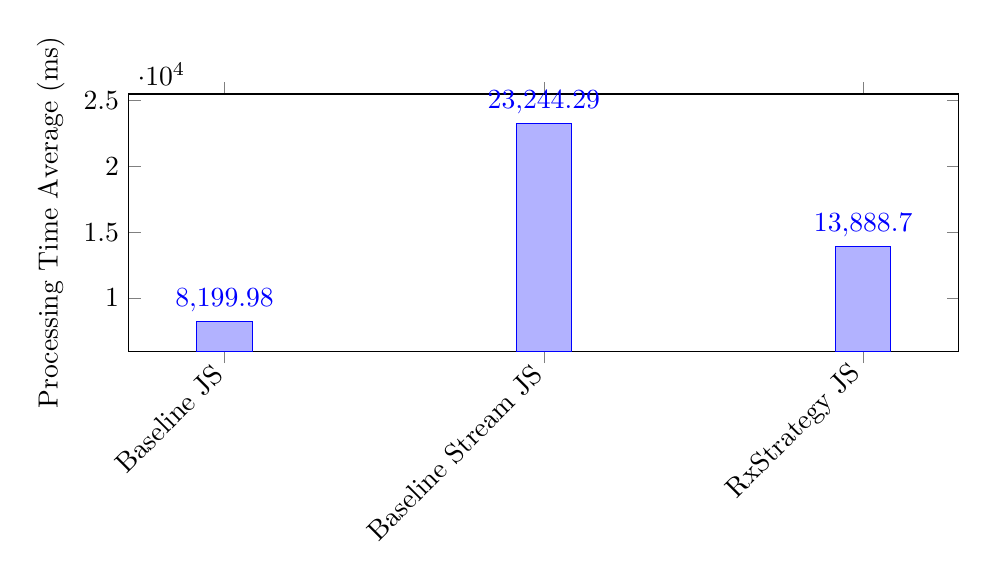
\begin{tikzpicture}
    \begin{axis}[
        ybar=2*\pgflinewidth,
        width=1.0\textwidth,
        height=0.4\textwidth,
        bar width=20pt,
        enlargelimits=0.15,
        legend style={at={(0.5,-0.2)}, anchor=north, legend columns=-1},
        ylabel={Processing Time Average (ms)},
        symbolic x coords={Baseline JS, Baseline Stream JS, RxStrategy JS},
        xtick=data,
        xticklabel style={rotate=45,anchor=east},
        nodes near coords,
        nodes near coords align={vertical},
        ]
    \addplot coordinates {(Baseline JS, 8199.98) (Baseline Stream JS, 23244.29) (RxStrategy JS, 13888.70)};
    \end{axis}
    \end{tikzpicture}
    \caption{Processing times for different JavaScript strategies for "Biggest Word".}
    \label{fig:biggest_word_processing_times_js}
\end{figure}



\subsection{Discussion}
\label{subsec:discussion}

% Here you discuss the results, as you did in the provided document.



\section{Conclusion}
\label{sec:conclusion}

\end{document}